%%%%%%%%%%%%%%%%%%%%%%% file template.tex %%%%%%%%%%%%%%%%%%%%%%%%%
%
% This is a general template file for the LaTeX package SVJour3
% for Springer journals.          Springer Heidelberg 2010/09/16
%
% Copy it to a new file with a new name and use it as the basis
% for your article. Delete % signs as needed.
%
% This template includes a few options for different layouts and
% content for various journals. Please consult a previous issue of
% your journal as needed.
%
%%%%%%%%%%%%%%%%%%%%%%%%%%%%%%%%%%%%%%%%%%%%%%%%%%%%%%%%%%%%%%%%%%%
%
% First comes an example EPS file -- just ignore it and
% proceed on the \documentclass line
% your LaTeX will extract the file if required
\begin{filecontents*}{example.eps}
%!PS-Adobe-3.0 EPSF-3.0
%%BoundingBox: 19 19 221 221
%%CreationDate: Mon Sep 29 1997
%%Creator: programmed by hand (JK)
%%EndComments
gsave
newpath
  20 20 moveto
  20 220 lineto
  220 220 lineto
  220 20 lineto
closepath
2 setlinewidth
gsave
  .4 setgray fill
grestore
stroke
grestore
\end{filecontents*}
%
\RequirePackage{fix-cm}
%
%\documentclass{svjour3}                     % onecolumn (standard format)
%\documentclass[smallcondensed]{svjour3}     % onecolumn (ditto)
\documentclass[smallextended]{svjour3}       % onecolumn (second format)
%\documentclass[twocolumn]{svjour3}          % twocolumn
%
\smartqed  % flush right qed marks, e.g. at end of proof
%
\usepackage{graphicx}
%
% \usepackage{mathptmx}      % use Times fonts if available on your TeX system
%
% insert here the call for the packages your document requires
%\usepackage{latexsym}
% etc.
%
% please place your own definitions here and don't use \def but
% \newcommand{}{}
%
% Insert the name of "your journal" with
% \journalname{myjournal}
%
\begin{document}

\title{Developing a parsimonius predictor for binary traits in sugar
  beet (\emph{Beta vulgaris}) \thanks{Filippo Biscarini and Nelson Nazzicari contributed
    equally to the work.}
}
%\subtitle{Do you have a subtitle?\\ If so, write it here}

\titlerunning{Parsimonious predictor for binary traits in sugar beet}        % if too long for running head

\author{Filson Nazzarini         \and
        Simone Marini \and
	Piergiorgio Stevanato \and
	Nelppo Biscicari %etc.
}

%\authorrunning{Short form of author list} % if too long for running head

\institute{F. Biscarini \at
              Fondazione Parco Tecnologico Padano \\
              %Tel.: +123-45-678910\\
              \email{filippo.biscarini@tecnoparco.org}           %  \\
%             \emph{Present address:} of F. Author  %  if needed
 \and
 S. Marini \at
    Dipartimento di Ingegneria Industriale e dell'Informazione \\
    Universit\`{a} di Pavia
	\and
	N. Nazzicari \at
    Fondazione Parco Tecnologico Padano \\
    %Tel.: +123-45-678910\\
    \email{nelson.nazzicari@tecnoparco.org}           %  \\
	\and
	P. Stevanato \at
	DAFNE, Universit\`{a} di Padova \\
        24105 Padova, Italy
}


\date{Received: 05 August 2014 / Accepted:}
% The correct dates will be entered by the editor

\maketitle

\begin{abstract}
Insert your abstract here. Include keywords, PACS and mathematical
subject classification numbers as needed.
\keywords{binary traits \and genomic predictions \and parsimonious predictor \and sugar beet}
% \PACS{PACS code1 \and PACS code2 \and more}
% \subclass{MSC code1 \and MSC code2 \and more}
\end{abstract}

\section{Introduction}
\label{intro}
The primary goal of breeding schemes in farm animals and crops is
generally to increase the agricultural output. Production traits are
typically quantitative continuous variables (e.g. milk
yield in dairy cattle, or per hectare yield in maize and rice).
Many traits of importance in plant and animal breeding follow nonetheless
a discrete categorical distribution, both ordered (e.g. calving ease in
cattle, grain texture in rice) and unordered
(e.g. grain pigmentation in rice, coat colour in cattle). A special case
is that of binomial traits, which can take up only two different values,
like disease resistance/susceptibility or presence/absence of a
morphological characteristic. 
Annual bolting (flowering) behaviour and root vigor are examples of binomial traits of agronomic
importance in sugar beet (\emph{Beta vulgaris}). [move this?] 

Advances in biotechnology and genomics, and the advent of high-density
molecular markers (especially sinlge-nucleotide polymorphisms, SNP)
genotyping have led to the emergence of molecular breeding
\cite{moose2008molecular}.
One exciting application of molecular breeding is genomic selection: the possibility of predicting the genetic value and future
performance of selection candidates solely from their genotypes (\cite{meuwissen2001prediction}). The predictive equations are
trained on reference individuals with both genotypic and phenotypic data and then
applied to selection candidates with genotypes only. Genomic selection
may bring about multiple benefits in breeding programmes such as
shorter breeding cycles or more efficient (e.g. traits difficult or
expensive to phenotype) and more accurate (e.g. traits with low
heritability) estimation of breeding values/selection
(\cite{goddard2007genomic,heffner2010plant}).
Key to the application of genomic selection to breeding programmes are reliable genomic
predictions.
The recent publication of the reference genome for \emph{Beta
vulgaris} genome \cite{dohm2013genome} is facilitating the application
of molecular breeding also in this crop species. Pioneering studies on
genomic predictions for both continuous (\cite{hofheinz2012genome,wurschum2013genomic}) and binary
(\cite{biscarini2014genome}) traits in sugar beet have already been published.

Genomic predictions are being based on increasing number of molecular
markers (e.g. 777K SNP-chip in cattle, 56K SNP-chip in maize,
whole-genome sequence data). When a huge number of potential predictors
is available, it may be useful to select a subset to limit laboratory
and bioinformatics costs, and the time of analysis, while at the same
time improving interpretability of results. There is therefore interest
in finding the minimum necessary set of information for a specific
problem. The principle of parsimony states that
a model needs to be simpler than the data the it explains (think for
instance of K-nearest neighbors -KNN- classifier with k=1), and according to Occam's razor, given two models that explain the data
equally well, the simplest has to be chosen (\cite{chaitin2006limits}).

The objective of this paper is to present the development of a
parsimonious predictor for the binary trait root vigor in a population
of sugar beet accessions.
SNPs in the panel were ranked based on their relevance and used to classify observations: one SNP at a
time was removed, progressively reducing the number of SNPs in the
predictive model.
We found that it was possible to strongly reduce the dimension of the
predictor and still achieve high accuracy.


\section{Material and methods}

\subsection{Plant material and SNP genotypes}
\label{sec:data}
A population of 124 individual sugar beet (\emph{B. vulgaris}) plants
from 18 high- and low-root-vigor lines were available. These lines were
characterised by different productivity and were provided by Lion Seeds
Ltd. (UK). Root vigor is related to nutrient uptake from the soil and plant productivity
(\cite{stevanato2010root}), and is recorded as a binary trait (either
high or low). The lines	were phenotyped	by measuring the root
elongation rate of eleven-days-old seedlings grown under hydroponic
conditions. There was no predetermined root
elongation rate threshold to classify a sugar beet as having high or low
root vigour, and the decision was subjectively made upon phenotypic
inspection. The classification has nevertheless been shown to be robust:
seedlings classified as "low" or "high" maintain the same class also at the
adult plant stage (\cite{stevanato2010root}). 
There were three low-root-vigor (24 individuals)
and 15 high-root-vigor (100 individuals) lines. Root elongation rate was
$< 3$ mm/day in the low-root-vigor lines and $>6$ mm/day in the
high-root-vigor lines.

All individual plants were genotyped for 192 SNP markers with the
high-throughput marker array QuantStudio 12K Flex system
coupled with Taqman OpenArray technology. Additional details on the
genotyping procedure are described in Stevanato et al., 2013 (\cite{stevanato2013high}).

The initial genotype screening led to the detection of one duplicated
individual ($100\%$ matching genotypes) from a high-root-vigor line,
which was removed. The average per-sample
and per-marker call-rate was $0.984$ and $0.969$. Only one SNP had a
per-marker call-rate $\leq 85\%$ and was removed from the analysis.
% There were in total 738  missing
% genotypes ($3.14\%$). Missing genotypes were imputed based on
% linkage disequilibrium (LD, \cite{browning2007rapid}).
After imputation data were edited for
minor allele frequency (MAF): 16 SNPs with MAF $\leq 2.5\%$ were
discarded. This left a total of 123 individuals and 175 SNP markers for
the analysis.
An overview of the data used in the paper is given in
% Table~\ref{tab:overview}. Table~\ref{tab:chromosome} reports the
% distribution of the 175 SNPs (and related scaffolds) used in the
% analysis along the 9 chromosomes of the \emph{Beta
%   vulgaris} genome. The average scaffold size was $1037$ kbps
% (range: $34.5$ - $4957$ kbps). 

Root vigor. Available data. SNP technology used, imputation. \\
Copypaste from other articles. Dataset description.
Text with citations \cite{stevanato2013high} and
\cite{saccomani2009molecular}.

\subsection{Predictor development procedure}
\label{sec:overview}
A two-step approach was adopted for the construction of a parsimonious
predictor for root vigor.

- a ranker to rank the various available predictors (SNPs in our case). We
  used the BOSS algorithm
- this is an iterative step. we progressively reduced the predictors set, 
  taking away the laest useful predictor and applying to the resulting
  subset a ridge logistic regression apprach. Thus, we obtained as many
  performances estimation as the number of original predictors.
\subsubsection{Rank of predictors}
\label{par:boss}
This explain the BOSS algorithm \cite{russu2012stochastic}

\subsubsection{Selection of predictors and classification method}
\label{par:predictor_selection}
We take one predictor out at each iteration
You put the model formula for ridge logistic regression

\subsubsection{Predictive ability}
\label{par:estimating_error}
Cross validation: how many times, what fractions. 
Explanation of error rate and other parameters (ROC?)

\subsection{Comparison with another method to rank predictors}
\label{sec:other_ranker}
Another ranker: why use one, and its description.
P value and SNP effect (as it is done in GWAS)

SNP variance \cite{gianola2009additive}

\subsection{Software}
\label{sec:software}
R \cite{r2008manual}, weka \cite{hall2009weka}, perl.

\section{Results}
\label{sec:results}

Figure~\ref{fig:accuracy}: Accuracy as a function of the number of
predictors, BOSS vs logistic [improve plot: no need to go down to 0.0 in
the y-axis; legend names and position; color of the lines? The ``bump''
at around 20-30 SNPs is not visible]

Table~\ref{tab:error}: TER, FPR, FNR for the first 30/35 SNPs + average for the
rest of the SNP (error close to $0$). BOSS + GWAS (6 columns)


Probability of assignment as a function of predictors:
Figure~\ref{fig:probability}. Better a table? Maybe in discussion?

From ROC curves only the AUC. No plot, use AUC as result in the text (e.g.
comparison between ranker: overall average AUC, average AUC per \# SNPs
+ std). Table?

% For one-column wide figures use
\begin{figure}
% Use the relevant command to insert your figure file.
% For example, with the graphicx package use
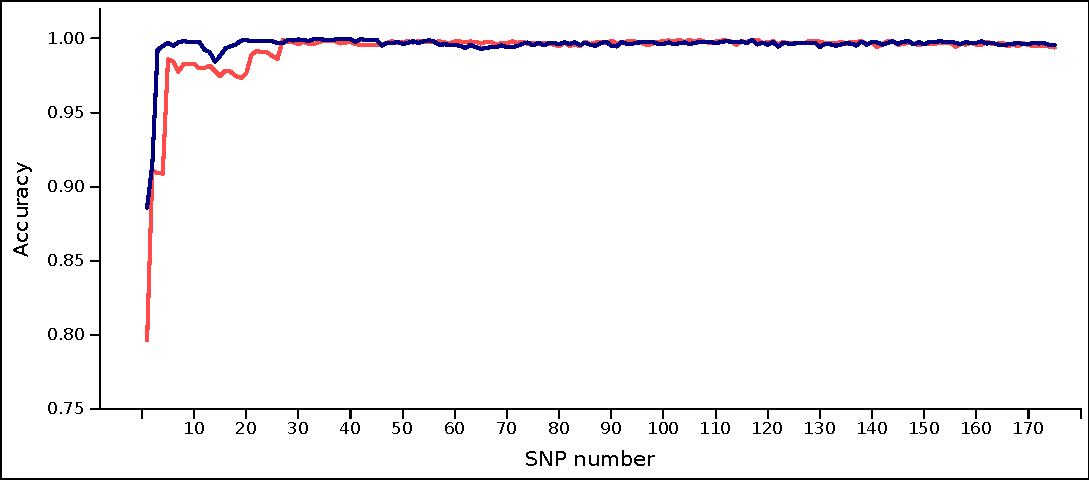
\includegraphics[width=0.95\textwidth]{accuracy.pdf}
% figure caption is below the figure
\caption{Accuracy (1 - error rate) of prediction as a function of the
  number of SNPs included in the classifier: BOSS (blue line) vs
  logistic regression (red line)}
\label{fig:accuracy}       % Give a unique label
\end{figure}

\begin{figure}
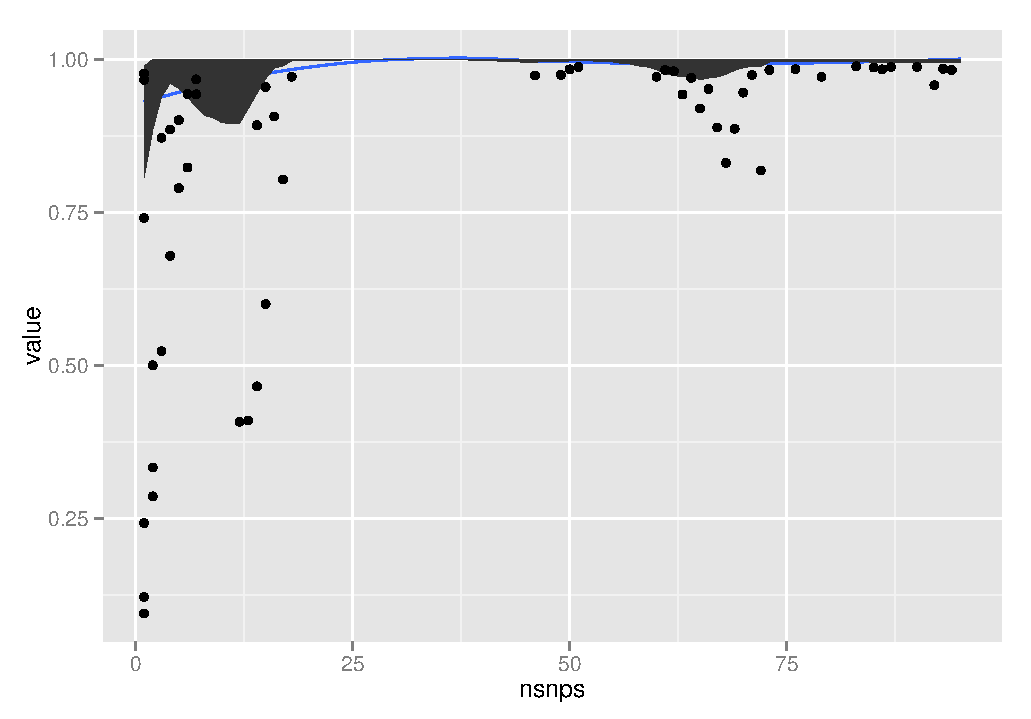
\includegraphics[width=0.95\textwidth]{prob_roll3.pdf}
\caption{Distribution of $P(Y=1|x)$ as a function of the number of SNPs
  in the classifier}
\label{fig:probability} 
\end{figure}


\section{Discussion}
\label{sec:discussion}
General overview
why error rates are not evenly distributed?
Reminder: it works very well because of LD and H2

Unstable below 30/40 SNPs; little ``bump'' around 20 SNPs: more marked
with BOSS, but also visible with GWAS. Why there? SNPs with large effect
on the trait, but low significance? SNPs with large effect but low LD
(with the QTL)? In the latter case, the marker might sometimes be in the
opposite phase. Look also at marker frequency.

Based on results, a panel of 30-35-40 SNPs is recommended for accurate
prediction of root vigor (move to breeding applications? Together with
development of a custom-chip?)

\subsection{Relative performance of rankers}
why using Pvalues and not other standard rankers (e.g. backward stepwise
selection)? Because of the specific nature of the problem

Comparison of rankers: spearman correlation + plot (ranker1 vs ranker2).

Figure~\ref{fig:rank}

\begin{figure}
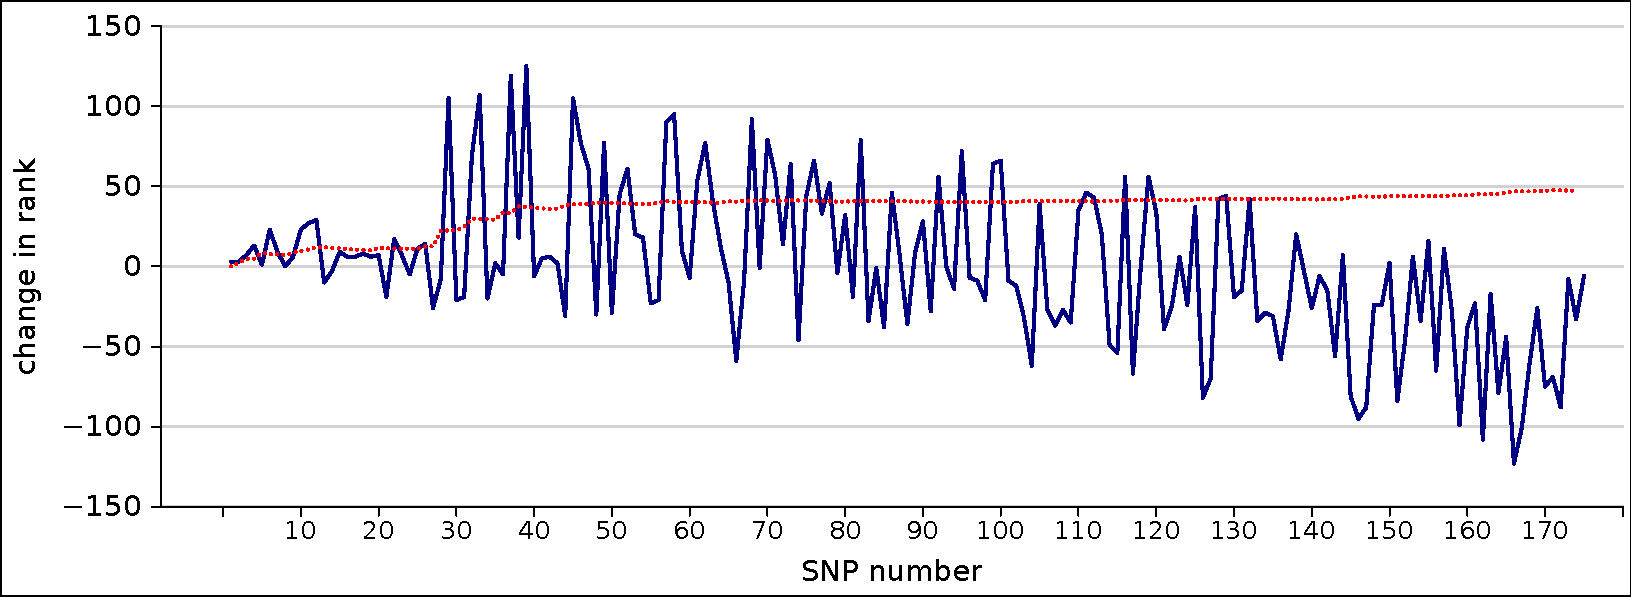
\includegraphics[width=0.95\textwidth]{rank.pdf}
\caption{Comparison of BOSS and logistic regression in terms of relative
rank position of relevant SNPs}
\label{fig:rank} 
\end{figure}


\subsection{SNP effects}
Manhattan plot with BOSS weights and weights from the other articles,
somehow compared (same chart? two charts? only ten best?).

Do the peaks make sense from the biological perspective?

Variance of SNPs vs genetic variance: $\rightarrow$ missing
heritability? (cite Brachi 2011, Manolio 2009?).

BOSS probability: 1 big peak + smaller peaks. Compare against SNP
density? Maybe the big peak corresponds to a physically isolated SNP,
whereas smaller peaks correspond to a cluster of SNPs in LD which
individually account for a smaller part of the variatino, but together
play an important predictive role. 


\subsection{Genotyping strategies and applications to breeding}
genotyping strategies: 
Costs, possible technologies (gbs, snp chip, macroarrays), implications

applications to breeding:
why is it important root vigor early detection. Other binomial traits (e.g.
disease resistance) May be applied to bolting (another trait which
exhibits binomial distribution), which has been shown to be controlled
by multiple genes and influenced by environmental factors
(\cite{salah2012genetic}).

sugar beet: $30\%$ of world's sugar production (cite Dohm? FAO?). Root
vigor linked to yield.

Sugar beet: sugar + energy (citation?)

Other binomial traits: resistance to viral and fungal diseases, bolting
(cite Dohm? Someone else?)

Breeding has shaped the genome of sugar beet (comparison with \emph{Beta
  maritima}, \cite{dohm2013genome}).

Extensions to multinomial traits? Examples?

potential and challenges of genomic selection in plant breeding (\cite{jonas2013does})

% For two-column wide figures use
%\begin{figure*}
% Use the relevant command to insert your figure file.
% For example, with the graphicx package use
%  
\includegraphics[width=0.75\textwidth]{example.eps}
% figure caption is below the figure
%\caption{Please write your figure caption here}
%\label{fig:2}       % Give a unique label
%\end{figure*}
%

\section{Conclusions}
\label{sec:conclusions}

Concluding remarks. 


\begin{acknowledgements}
This research was financially supported by the Marie Curie European
Reintegration Grant ``NEUTRADAPT''.
\end{acknowledgements}

%\section{Tables}

% For tables use
\begin{table}
% table caption is above the table
\caption{Total error rate (TER), false positive (FPR) and false negative
  (FNR) rates as a function of the number of SNPs ranked according to
  BOSS or logistic regression}
\label{tab:error}       % Give a unique label
% For LaTeX tables use
\begin{tabular}{cccc}
\hline\noalign{\smallskip}
\# SNPs & TER & FPR & FNR \\
\noalign{\smallskip}\hline\noalign{\smallskip}
1 & 0.114 & 0.065 & 0.049 \\
2 & 0.085 & 0.037 & 0.047 \\
3 & 0.008 &  &  \\
4 & 0.005 &  &  \\
5 & 0.003 &  &  \\
6 & 0.005 &  &  \\
7 & 0.003 &  &  \\
8 & 0.002 &  &  \\
9 & 0.003 &  &  \\
10 & 0.002 &  &  \\
11 & 0.002 &  &  \\
12 & 0.008 &  &  \\
13 & 0.009 &  &  \\
14 & 0.016 &  &  \\
15 & 0.012 &  &  \\
16 & 0.007 &  &  \\
17 & 0.005 &  &  \\
18 & 0.004 &  &  \\
19 & 0.002 &  &  \\
20 & 0.001 &  &  \\
\dots & \dots &  \dots &  \dots \\
21--30 & 0.002  &  &  \\
31--40 & 0.001 &  &  \\
41--100 & 0.003 &  &  \\
101--175 & 0.001 &  &  \\
\noalign{\smallskip}\hline
\end{tabular}
\end{table}


% BibTeX users please use one of
%\bibliographystyle{spbasic}      % basic style, author-year citations
\bibliographystyle{spmpsci}      % mathematics and physical sciences
%\bibliographystyle{spphys}       % APS-like style for physics
\bibliography{parsimonious.bib}   % name your BibTeX data base

% Non-BibTeX users please use
%\begin{thebibliography}{}
%
% and use \bibitem to create references. Consult the Instructions
% for authors for reference list style.
%
%\bibitem{RefJ}
% Format for Journal Reference
%Author, Article title, Journal, Volume, page numbers (year)
% Format for books
%\bibitem{RefB}
%Author, Book title, page numbers. Publisher, place (year)
% etc
%\end{thebibliography}

\end{document}
% end of file template.tex

